O objetivo desta seção é descrever a replicação em si, do arcabouço de captura de
ativações até a comparação contra os \textit{baselines} de extração mais baratos. Para
cada um dos 6 blocos do modelo registramos \textit{hooks} de passagem direta, capturamos a
saída $[B, T, 384]$ de cada bloco e extraímos a linha do último \textit{token} não
preenchido por \textit{padding} de cada \textit{prompt}, o que resulta em
$A \in \mathbb{R}^{n \times 6 \times384}$. Verificou-se o arcabouço quanto ao
determinismo, com \verb|model.eval()|, e quanto à invariância ao preenchimento, isto é, a
ativação de um \textit{prompt} independe do comprimento do preenchimento à direita,
propriedade que verificamos à ordem de $7\times 10^{-7}$.

\subsection{Conjuntos de dados dos conceitos}

Uma vez que as entradas cruas do usuário são fortemente moldadas por \textit{templates},
com apenas cerca de 4 a 34 cadeias únicas por categoria, utilizamos o diálogo ChatML
completo, ou seja, o turno do usuário junto à resposta do GuppyLM, como \textit{prompt}, o
que resulta em centenas de textos distintos por categoria. Sobre eles construímos três
conceitos binários, cada um deles definido como um contraste entre grupos de categorias,
conforme reportado na Tabela~\ref{tab:concept_categories}.


\begin{table}[htbp]
\centering
\caption{Os três conceitos binários, definidos como contrastes entre categorias.}
\label{tab:concept_categories}
\begin{tabular}{@{}l p{4.2cm} p{4.6cm} c@{}}
\toprule
\textbf{Conceito}& \textbf{Categorias positivas} & \textbf{Categorias negativas} & \textbf{N/classe} \\
\midrule
food &  food, taste & weather, seasons, tv, music, glass, rain, outside & 300 \\
valence &  happy, excited, love, curious & scared, fear, bored, tired & 100 \\
env\_social &  water, filter, temp\_hot, temp\_cold, algae & greeting, bye, friends, visitors, lonely & 300 \\
\bottomrule
\end{tabular}
\end{table}

Cada conceito é balanceado entre classes e dividido em 60/20/20 nos conjuntos de
treinamento, validação e teste sobre as cadeias de diálogo \emph{únicas}, com a ausência
de vazamento de \textit{prompts} entre as partições assegurada no momento da construção.
Isso fornece 360/120/120 exemplos para \verb|food| e \verb|env_social|, e 120/40/40 para
\verb|valence|. Note que \verb|valence| é, portanto, o menor dos três conceitos por um
fator de três, fato que vale manter em mente na leitura de seus resultados adiante, uma
vez que toda diferença reportada para esse conceito repousa sobre uma amostra
proporcionalmente menor.

\subsection{Implementação da RFM}

A RFM foi implementada como um pacote Python, \verb|rfm_guppy|. As funções de seu núcleo,
a saber, \verb|laplace_kernel|, \verb|rfm_fit|, \verb|agop_grad|, \verb|top_eigvectors|,
\verb|orient| e \verb|extract_concept_vector|, realizam a extração do vetor de conceito
utilizando entradas centradas na média, gradientes vetorizados da AGOP com a proteção para
$d_i = 0$, \verb|eigh| sobre a matriz PSD $384 \times 384$, e seleção de hiperparâmetros
pela maximização do $|\rho|$ de validação, isto é, o valor absoluto da correlação de
Pearson entre $\langle a, v \rangle$ e $y$, sobre $\sigma \in \{1, 10, 100\}$,
$T \in \{1, \dots, 10\}$ e $\mathrm{normalize} \in \{\mathrm{False}, \mathrm{True}\}$.

Escrever o gradiente de todos os pontos de treinamento de uma só vez, como um tensor
$[n, n, k]$, custaria cerca de 400\,MB, de forma que o reescrevemos como um par de
produtos matriciais. Definimos

\[
  W_{ij} = \frac{\alpha_j \, K_M\!\left(a^{(i)}, a^{(j)}\right)}
                {\sigma \, d_j\!\left(a^{(i)}\right)},
  \qquad
  W_{ij} = 0 \ \text{ quando } d_j\!\left(a^{(i)}\right) = 0,
\]

de modo que a matriz de gradientes empilhados $G \in \mathbb{R}^{n \times k}$, cuja
$i$-ésima linha é $\nabla_z f_t(a^{(i)})^{\top}$, é dada por

\[
  G = -\left(\operatorname{diag}\!\left(W \mathbf{1}\right) Z_c \;-\; W Z_c\right) M ,
\]

com $\mathbf{1} \in \mathbb{R}^{n}$ o vetor de uns e $Z_c$ as ativações centradas na
média. O pico de memória é então $O(nk + n^2)$, e não $O(n^2 k)$. A varredura sobre $T$
também é executada incrementalmente, no sentido de que a iteração $T+1$ prossegue a partir
da matriz $M$ obtida na iteração $T$.

Antes de rodar sobre dados reais, submetemos a implementação a um teste de recuperação
sintética. Geramos $n = 1000$ pontos normais padrão $z_i \in \mathbb{R}^{k}$ com $k = 384$
e os rotulamos por $y_i = \langle z_i, u \rangle$ para uma direção oculta $u$ com
$\|u\|_2 = 1$, e confirmamos em seguida que o autovetor principal $v$ retornado pela RFM
se alinha com $u$. O critério de aceitação pré-declarado é $|\cos(v, u)| > 0{,}90$, e a
execução atinge $|\cos(v, u)| = 0{,}9528$.

Dois detalhes desse teste são deliberados. Em primeiro lugar, os 1.000 pontos são
divididos em 800/200 entre treinamento e validação, de forma que o $|\cos(v,u)|$ reportado
seja obtido dos hiperparâmetros que maximizam o $|\rho|$ de validação, exatamente como nos
conceitos reais. Em segundo lugar, os rótulos aqui são de valor real, e não os
$y \in \{0,1\}$ da §2, uma vez que recuperar uma direção em $\mathbb{R}^{384}$ a partir de
800 pontos é uma pergunta sobre a maquinaria da AGOP, e limiarizar $\langle z, u \rangle$
em um sinal descartaria a maior parte da informação sobre $u$, a menos que $n \gg k$. Note
que o teste é, portanto, um problema mais fácil do que os conceitos que se seguem, por
construção, o que significa que ele é uma verificação de correção da implementação e não
um referencial de dificuldade. O comportamento da recursão nesse teste é apresentado na
Figura~\ref{fig:agop_convergence}.

\begin{figure}[htbp]
    \centering
    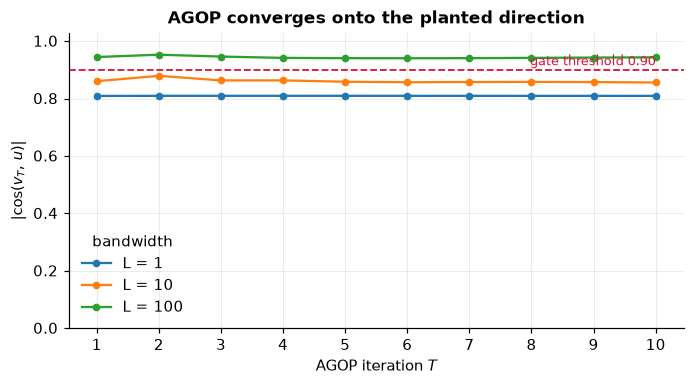
\includegraphics[width=0.75\textwidth]{imgs/02_agop_convergence.png}
    \caption{Ao desenrolar manualmente o laço da AGOP, vê-se que a curva de convergência é plana.}
    \label{fig:agop_convergence}
\end{figure}

O que é plano aqui é a \emph{recursão}, e não a AGOP. Uma vez que $T$ conta os passos
tomados a partir de $M_0 = I$, o vetor em $T = 1$ já é uma AGOP completa, formada dos
gradientes de um preditor ajustado com o \textit{kernel} de Laplace ordinário, e, como $y$
é exatamente linear em $\langle z, u \rangle$, esse único passo basta. É possível perceber
que $\sigma = 100$ alcança $|\cos(v,u)| = 0{,}945$ em $T = 1$ e que as nove iterações
seguintes não alteram nada, enquanto $\sigma = 1$ permanece em $0{,}809$ e $\sigma = 10$ em
$0{,}860$, e nenhum dos dois consegue subir dali. O que a varredura compra nesse teste é,
portanto, a \emph{largura de banda}, e não a contagem de iterações, o que é exatamente a
razão pela qual $\sigma$ é varrido aqui ao invés de copiado de Beaglehole et al. A
iteração justifica sua existência sobre ativações reais, onde ela leva $M$ em direção ao
posto 1\footnote{Posto($M$) = o número de autovalores não nulos daquela matriz. Quando $M$
tem posto 1, um autovalor é não nulo e todos os demais são zero, o que equivale a dizer
que $M$ se fatora como um único produto externo $M = \lambda_1 v_1 v_1^{\top}$ com
$\|v_1\|_2 = 1$}, o que é matéria distinta de encontrar a direção em primeiro lugar.

\subsection{Extração dos vetores de conceito}

Rodando a RFM para a extração dos conceitos, obtemos uma forte separabilidade linear para
todo conceito e em todo bloco, à exceção do primeiro deles, conforme reportado na
Tabela~\ref{tab:rfm-val-pearson}.

\begin{table}[htbp]
\centering
\caption{$|\text{Pearson}|$ de validação (RFM), por bloco}
\label{tab:rfm-val-pearson}
\begin{tabular}{c c c c}
\toprule
\textbf{Bloco} & \textbf{food} & \textbf{valence} & \textbf{env\_social} \\
\midrule
0 & 0{,}906 & 0{,}507 & 0{,}735 \\
1 & 0{,}973 & 0{,}899 & 0{,}941 \\
2 & 0{,}975 & 0{,}908 & \textbf{0{,}950} \\
3 & \textbf{0{,}978} & 0{,}905 & 0{,}944 \\
4 & 0{,}977 & \textbf{0{,}918} & 0{,}942 \\
5 & 0{,}977 & 0{,}908 & 0{,}943 \\
\bottomrule
\end{tabular}
\end{table}

Note que o bloco 0 é consistentemente mais fraco para todo conceito, o que sugere que um
único bloco de atenção e MLP não é suficiente para construir a característica, enquanto os
blocos 1--5 todos fornecem uma projeção fortemente correlacionada com o rótulo. Os
conceitos \verb|food| e \verb|env_social| são distinções de tópico, exatamente o tipo de
coisa que um modelo pequeno codifica de forma tosca, ao passo que \verb|valence| é o mais
fraco em toda a extensão, e isso é em si um achado, uma vez que o mecanismo não reporta o
mesmo sucesso em todo conceito que lhe é entregue, o que é o que se deseja de uma medição,
e não de uma demonstração.

\begin{figure}[htbp]
    \centering
    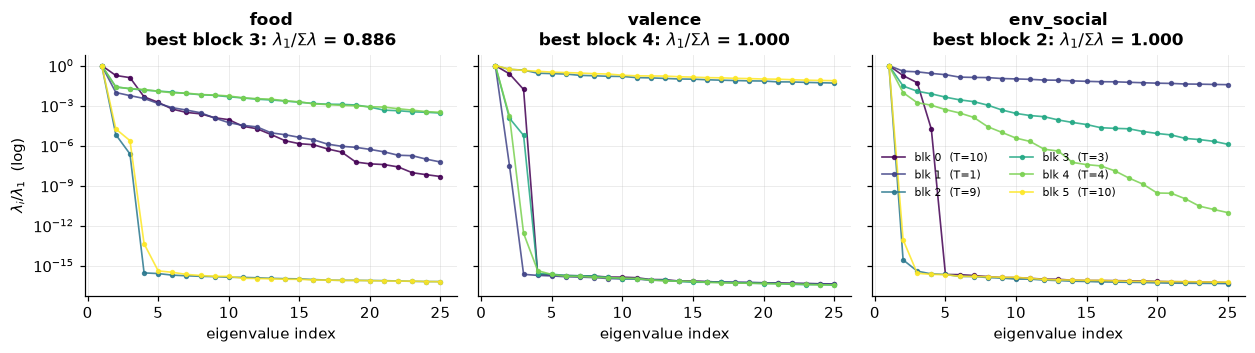
\includegraphics[width=0.75\textwidth]{imgs/03_agop_spectra.png}
    \caption{Quão de posto 1 são os conceitos?}
    \label{fig:agop_spectra}
\end{figure}

Passamos também a estudar o quanto os conceitos são de posto 1, utilizando duas
quantidades distintas. A curva da Figura~\ref{fig:agop_spectra} é o espectro normalizado
$\lambda_j / \lambda_1$ contra o índice do autovalor $j$, enquanto a estatística resumo
citada abaixo é $\lambda_1 / \sum_j \lambda_j$, a fração da massa espectral carregada pela
direção principal. Cada bloco é traçado na iteração $T$ que a varredura de validação
selecionou para ele, e o espectro depende fortemente desse $T$. Onde a varredura escolheu
muitas iterações, o colapso é praticamente total, como em \verb|env_social| no bloco 2,
selecionado em $T = 9$, que possui $\lambda_2 / \lambda_1 \approx 3 \times 10^{-15}$, isto
é, numericamente de posto 1. Onde ela escolheu $T = 1$, a matriz mal foi reponderada e o
espectro permanece largo, como em \verb|valence| no bloco 5, que se situa em
$\lambda_1 / \sum_j \lambda_j = 0{,}147$. No bloco em que o $|\rho|$ de validação é o mais
alto para cada conceito, $\lambda_1 / \sum_j \lambda_j$ vale $0{,}886$ (\verb|food|, bloco
3), $1{,}000$ (\verb|valence|, bloco 4) e $1{,}000$ (\verb|env_social|, bloco 2), de forma que
ali o conceito é realmente uma única direção. Note que esse bloco é reportado apenas para
fins descritivos, uma vez que o \textit{steering} perturba todos os seis blocos ao mesmo
tempo, cada um com o seu próprio $v_\ell$, e a \textit{probe} de \textit{monitoring} lê todos os
seis, de modo que nada a jusante seleciona sobre ele.

A observação mais interessante é que as duas propriedades se descolam. O conceito
\verb|valence| no bloco 2 possui um $M$ completamente não degenerado, com
${\lambda_1}/{\sum \lambda} = 0{,}186$, e ainda assim alcança um $|\rho|$ de validação de
$0{,}908$, essencialmente igualando a solução de posto 1 do bloco 4, em $0{,}918$. Concluímos,
portanto, que a concentração do espectro da AGOP não é um pré-requisito para que o
autovetor principal seja uma boa direção de conceito, pois a direção é recuperável muito
antes de $M$ ter terminado de colapsar sobre ela.

\subsection{\textit{Steering}}

Voltamo-nos agora ao \textit{steering} em si, e a lição mais interessante que encontramos é
que quem quer que deseje aplicá-lo a um modelo não deve reutilizar cegamente os
coeficientes de Beaglehole et al. Os valores $\varepsilon \in \{0{,}1; \ldots; 0{,}65\}$ ali
reportados são calibrados para a escala de ativações do Llama, ao passo que as normas de
ativação do GuppyLM são de 12 a 31, de forma que $\varepsilon$'s tão pequenos fariam muito
pouco. Escolhemos, ao invés disso,

\[
  \varepsilon_\ell = r \cdot \operatorname*{median}_{i} \left\| a_\ell^{(i)} \right\|_2 ,
\]

sendo a mediana tomada sobre todas as ativações de treinamento armazenadas, agregadas
entre os três conceitos. Como $\|v_\ell\|_2 = 1$, o coeficiente relativo $r$ é exatamente
o tamanho da perturbação como fração da norma típica do fluxo residual naquele bloco, e é
$r$, e não $\varepsilon$, que se transporta entre modelos. Varremos
$r \in \{-4;\, -2;\, -1;\, -0{,}5;\, -0{,}25;\, 0;\, +0{,}25;\, +0{,}5;\, +1;\, +2;\, +4;\, +8\}$.
Note que o truque aqui é o \textit{hook}, pois retornar um tensor de um \textit{hook} de
passagem direta do PyTorch substitui a saída do módulo, e o \textit{hook} dispara a cada
\textit{token} gerado. A Tabela~\ref{tab:steering_samples} apresenta gerações de exemplo
para o \textit{prompt} de sondagem ``How are you doing today?''.

\begin{table}[htbp]
\centering
\caption{Gerações de exemplo para o \textit{prompt} de sondagem \textit{``How are you doing today?''} (``Como você está hoje?'', em tradução livre) sob \textit{steering} em $r=0$ (linha de base) contra $r=+0{,}25$.}
\label{tab:steering_samples}
\small
\begin{tabular}{@{}l p{5.5cm} p{5.5cm}@{}}
\toprule
\textbf{Conceito} & \textbf{$r = 0$ (linha de base)} & \textbf{$r = +0{,}25$} \\
\midrule
food &
\textit{``i'm a little fish. i am small but i have opinions. mostly about food.''} &
\textit{``whole palate palate palate promise to promise to best excited palate best \ldots''} \\
\addlinespace
valence &
(mesma linha de base) &
\textit{``tv means floating someone wanting chestpick now either excited. noticed bit happ\ldots''} \\
\addlinespace
env\_social &
(mesma linha de base) &
\textit{``if can breathe can if breathe can if if i breathe breathe more breathe if if if\ldots''} \\
\bottomrule
\end{tabular}
\end{table}

A intervenção inequivocamente funciona, e é inequivocamente tosca. Uma direção ajustada
sobre pares $(\textit{prompt}, \text{rótulo})$, que jamais viu uma única geração, arrasta a
saída para um vocabulário de aquário e água a partir de um \textit{prompt} de sondagem que
não menciona nada disso, de forma que a afirmação causal se replica. Entretanto, ao se ler
o texto ao invés das palavras-chave, o que ali está é uma deriva de vocabulário repetitiva
e quase agramatical, e não um peixe fluente falando sobre seu aquário. Duas coisas
plausivelmente contribuem para isso, e não podemos separar nenhuma das duas com um único
modelo. A perturbação pode simplesmente ser maior do que a folga que um fluxo residual de
8{,}7M de parâmetros tem para absorver, e os vetores são ajustados sobre a ativação do
último \textit{token} de um diálogo ChatML \emph{completo}, enquanto o \textit{steering} os
escreve em toda posição de um diálogo \emph{parcial}, de modo que a direção está sendo
aplicada a uma distribuição de estados sobre a qual ela nunca foi estimada.

Pontuamos as intervenções de \textit{steering} sobre um conjunto de 7 \textit{prompts} de
sondagem neutros,
12 valores de $r$ e 3 conceitos pela taxa de acerto no léxico, e os três conceitos contam
histórias bastante distintas, conforme se pode ver na
Figura~\ref{fig:steering_lexicon_sweep}.

\begin{figure}[htbp]
    \centering
    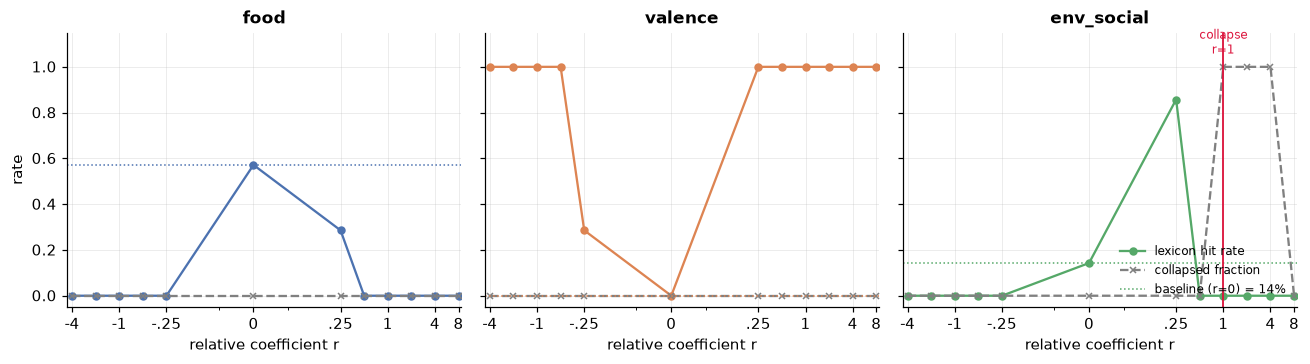
\includegraphics[width=0.75\textwidth]{imgs/04_steering_lexicon_sweep.png}
    \caption{Três formatos, três falhas distintas da métrica.}
    \label{fig:steering_lexicon_sweep}
\end{figure}

O conceito \verb|env_social| se comporta como Beaglehole et al. prediriam, indo de uma
linha de base de 14\% a 86\% em $r = +0{,}25$ e colapsando em seguida, com 7 de 7 gerações
degeneradas em $r = +1$, $+2$ e $+4$. Essa é uma faixa útil estreita com um teto duro,
exatamente o formato descrito, ainda que uma faixa magra, uma vez que os 14\% da linha de
base são uma única geração contendo \emph{hello} (olá), palavra tomada das categorias
\emph{negativas} do conceito, e os 86\% são uma única palavra-chave, \emph{cold} (frio),
aparecendo em 6 das 7 gerações. Note que nenhuma outra palavra do polo positivo dispara em
qualquer ponto da varredura.

O conceito \verb|food| falha por essa medida, e falha de forma instrutiva. Sua linha de
base em $r = 0$ já é de 57\%, porque um peixe cuja personalidade inteira é pensar em
comida menciona comida sem ser solicitado, e o \textit{steering} não pode acrescentar um
conceito que já está saturado, de modo que ele só pode quebrar as frases que o carregavam,
e a taxa de acerto consequentemente \emph{cai}, de 57\% para 29\% em $r = +0{,}25$ e depois
para 0\% em todo o resto. A queda em sua maior parte nem sequer é uma questão de fluência,
uma vez que a palavra que domina as gerações em $r = +0{,}25$ é \emph{palate} (paladar), com
56 ocorrências ao longo das sete saídas, o que está francamente dentro do conceito e
simplesmente ausente do léxico de treze palavras. O que essa curva mede é, portanto, a
lista de palavras-chave deixando escapar o vocabulário que o \textit{steering} produziu.

O conceito \verb|valence| reporta 100\% em $r = \pm 0{,}5$ e além, em ambas as direções. Isso
não é \textit{steering} simétrico, é a métrica escalar descartando um sinal que ela de fato
registrou. O léxico de \verb|valence| abrange os dois polos, com \emph{happy, excited, joy}
ao lado de \emph{scared, fear, tense, stiff, hide}, de forma que um empurrão em qualquer
sentido pontua um acerto, e ainda assim as palavras em si se separam de maneira limpa,
pois todo $r \leq -0{,}5$ dispara \emph{hide} (esconder-se) em 7 de 7 gerações e todo
$r \geq +0{,}25$ dispara \emph{excited} (animado) em 7 de 7, sem cruzamento algum. A
\emph{taxa} de acerto é cega ao sinal, os acertos não o são. Vale enunciar isso
claramente, pois trata-se de evidência bidirecional que não vem da \textit{probe}, e que
não está portanto sujeita à circularidade discutida adiante. A mesma construção de dois
polos se aplica a \verb|env_social|, cujo léxico também contém suas categorias negativas
(\emph{hello, hi, friend, bye}).

Uma ressalva é fácil de passar despercebida, e ela importa para a leitura de toda figura
``colapsada'' citada acima. O detector sinaliza uma geração apenas quando uma única
palavra toma mais de 60\% da saída, de forma que as gerações de \verb|food| em
$r = +0{,}25$, situadas entre 0{,}28 e 0{,}41 por essa medida, são sinalizadas como limpas
enquanto se leem como \emph{``whole palate palate palate promise to promise to best\ldots''},
e \verb|env_social| em $r = +8$ pontua 0{,}59 e é sinalizado como limpo enquanto produz a
mesma cadeia degenerada \emph{``if can breathe can if\ldots''} que pontua 0{,}61 e é
sinalizada como colapsada em $r = +4$. Note que um zero na coluna de colapso significa que
o texto não é maximamente repetitivo, mas não significa que o texto seja coerente.

O resultado honesto desta fase de \textit{steering} é que a direção é real e causal, e ainda
assim, em todo $r \neq 0$ que testamos, a fluência se degrada. Aparentemente um modelo de
8{,}7M de parâmetros tem folga pequena demais para absorver uma perturbação grande o
bastante para importar sem perder o fio da frase.

Para a avaliação do \textit{steering}, como não dispomos de um juiz GPT-4o nesta escala, a
segunda métrica é uma pontuação de \textit{probe}, obtida realimentando o texto gerado no
modelo como um diálogo ChatML completo e lendo a probabilidade do conceito reportada pela
\textit{probe} de \textit{monitoring}. Uma geração conta como sucesso de \textit{steering}
se a pontuação da
\textit{probe} é maior que 0{,}5 ou se ela acerta o léxico, e as taxas de sucesso
resultantes estão reportadas na Tabela~\ref{tab:steering_success}.

\begin{table}[htbp]
\centering
\caption{Taxa de sucesso do \textit{steering} (pontuação da \textit{probe} $>0{,}5$ ou acerto no léxico) em $r=0$ contra o melhor coeficiente positivo $r$ da varredura, por conceito.}
\label{tab:steering_success}
\begin{tabular}{@{}lccc@{}}
\toprule
\textbf{Conceito} & \textbf{Linha de base} & \textbf{Melhor} & \textbf{Melhor $r$} \\
\midrule
food        & 71{,}4\% & 100{,}0\% & $+0{,}25$ \\
valence     & 71{,}4\% & 100{,}0\% & $+0{,}25$ \\
env\_social & 28{,}6\% & 100{,}0\% & $+0{,}25$ \\
\bottomrule
\end{tabular}
\end{table}

\begin{figure}[htbp]
    \centering
    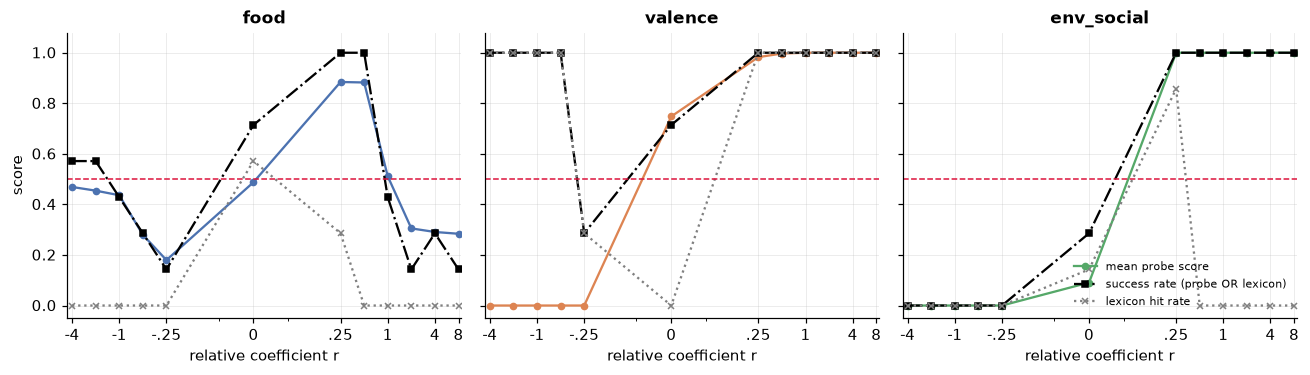
\includegraphics[width=0.75\textwidth]{imgs/05_steering_probe_sweep.png}
    \caption{A \textit{probe} (linha cheia) e o léxico (pontilhado) discordam em tudo aquilo que importa.}
    \label{fig:steering_probe_sweep}
\end{figure}

As ativações de fato se moveram, e fomos nós que as movemos ao aplicar o \textit{steering}, de
forma que esta métrica é parcialmente circular, dado que a \textit{probe} lê os autovetores
principais da AGOP e o vetor de \textit{steering} é ele próprio o autovetor principal da
AGOP. Em favor da \textit{probe}, ela não está meramente reagindo ao fato de ser
perturbada, uma vez que acompanha o sinal de $r$ em todos os conceitos (\verb|valence| e
\verb|env_social| caem a exatamente 0{,}00 sob \textit{steering} negativo e se mantêm em 1{,}00
sob \textit{steering} positivo, e mesmo \verb|food| separa a faixa de 0{,}18 a 0{,}47 sob
\textit{steering} negativo dos 0{,}88 em $r = +0{,}25$), o que é informação bidirecional genuína.
O que a \textit{probe} não consegue notar é que a frase que carregava aquela direção
deixou de ser uma frase. A cifra de 100\% não é, portanto, evidência independente de que o
\textit{steering} funciona, e não deve ser lida como tal.

\subsection{\textit{Monitoring}}

Utilizando os $p=3$ autovetores principais da AGOP por bloco, cada \textit{prompt} se torna
um vetor de projeções em $\mathbb{R}^{18}$, isto é, $6$ blocos vezes $3$ componentes, o que
constitui uma compressão de 128 vezes das ativações cruas $6 \times 384$. Uma
\textit{probe} de regressão logística, com um padronizador à frente e $C$ varrido na
validação, é treinada sob ambas as estratégias, a de melhor bloco e a agregada, e avaliada
sobre a partição de teste retida. Para todos os três conceitos a AUROC de teste é $1{,}000$.
A estratégia por bloco reporta o bloco 1 como o melhor para cada um deles, mas isso é um
desempate e não um resultado, uma vez que na validação os blocos 1--5 todos pontuam
exatamente $1{,}000$ e apenas o bloco 0 é mais fraco ($0{,}998$ para \verb|food|, $0{,}913$ para
\verb|valence| e $0{,}939$ para \verb|env_social|), de forma que o bloco 1 é meramente o
primeiro índice de um empate quíntuplo.

A separação é visível antes de qualquer classificador ser ajustado, como se pode ver ao
projetar a partição de teste sobre os dois primeiros autovetores da AGOP do melhor bloco de
cada conceito, o que é o que a Figura~\ref{fig:agop_projection_scatter} exibe.

\begin{figure}[htbp]
    \centering
    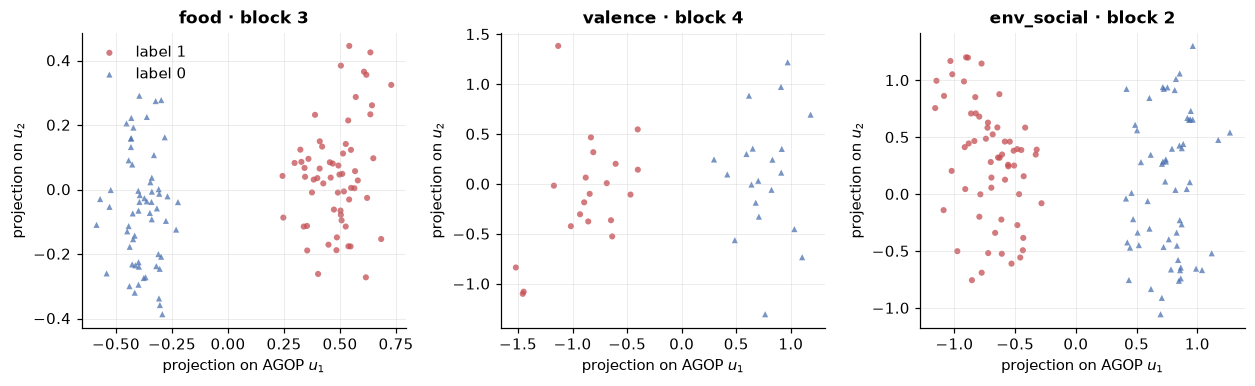
\includegraphics[width=0.75\textwidth]{imgs/06_agop_projection_scatter.png}
    \caption{Duas nuvens, separadas apenas pelo eixo horizontal.}
    \label{fig:agop_projection_scatter}
\end{figure}

A AUROC de teste é igual a 1{,}0 em toda a linha para ambas as estratégias, e toda curva ROC
é um ângulo reto. Mesmo uma única característica basta, pois o primeiro autovetor da AGOP
sozinho alcança uma AUROC de 1{,}0 sem auxílio nos três conceitos. O segundo e o terceiro
autovetores são muito mais fracos, com $u_2$ pontuando $0{,}679$, $0{,}617$ e $0{,}599$ e $u_3$
pontuando $0{,}519$, $0{,}645$ e $0{,}705$ em \verb|food|, \verb|valence| e \verb|env_social|
respectivamente. Note que quatro desses seis valores estão suficientemente acima de $0{,}5$
para se dizer que as direções secundárias carregam algum sinal residual de classe, o que é
uma pequena qualificação do quadro estritamente de posto 1, ao passo que o $u_3$ de
\verb|food| em $0{,}519$, sobre uma partição de teste de 120 exemplos, é indistinguível do
acaso.

Um teto não é a mesma coisa que um resultado forte, e três propriedades desta montagem a
tornam fácil. Os conceitos são as \emph{próprias} categorias de treinamento do modelo, e
não propriedades emergentes, as partições de teste são pequenas (120, 40 e 120 exemplos),
e as classes positiva e negativa são extraídas de grupos de categorias disjuntos e
claramente distintos. Uma quarta propriedade é específica ao modo como os dados foram
construídos, pois, como um \textit{prompt} é um diálogo completo contendo a própria
resposta do GuppyLM, a \textit{probe} está lendo o estado de último \textit{token} de um
texto que já enuncia lexicalmente o seu tópico, de forma que parte do que ela certifica é
classificação de tópico, e não a recuperação de um conceito latente. Uma pontuação perfeita
diz que o mecanismo de leitura linear está intacto a 8{,}7M de parâmetros, mas nada diz sobre
como o método se comporta em um conceito genuinamente difícil, porque nenhum lhe foi
apresentado.

\subsection{\textit{Baselines}}
\label{sec:baselines-anchor}

Rodamos PCA, DiffMeans, LogReg e RFM pelo mesmo \textit{pipeline},
isto é, as mesmas partições, a mesma \textit{probe}, o mesmo limiar de sucesso, e uma
varredura de \textit{steering} sobre
$r \in \{0;\, \pm 0{,}25;\, \pm 0{,}5;\, \pm 1;\, \pm 2\}$, mais estreita nos extremos que a
varredura de doze pontos utilizada acima, ainda que o melhor coeficiente positivo de todo
método caia em $r = +0{,}25$ e portanto bem dentro dela. A qualidade das direções obtidas por
cada método está reportada na Tabela~\ref{tab:baselines_val_rho}.

\begin{table}[htbp]
\centering
\caption{Qualidade das direções, $|\rho|$ de validação (correlação de Pearson com o rótulo) no melhor bloco de cada método.}
\label{tab:baselines_val_rho}
\begin{tabular}{@{}lccc@{}}
\toprule
\textbf{Método} & \textbf{food} & \textbf{valence} & \textbf{env\_social} \\
\midrule
PCA        & 0{,}929 & 0{,}154 & 0{,}490 \\
DiffMeans  & 0{,}975 & 0{,}800 & 0{,}914 \\
LogReg     & \textbf{0{,}986} & \textbf{0{,}960} & \textbf{0{,}972} \\
RFM        & 0{,}978 & 0{,}918 & 0{,}950 \\
\bottomrule
\end{tabular}
\end{table}

A separação predita por Beaglehole et al. de fato aparece, mas apenas contra a PCA, e
apenas nos dois conceitos mais difíceis, uma vez que a PCA desaba a 0{,}15 em \verb|valence|
contra os 0{,}92 da RFM e alcança 0{,}49 em \verb|env_social| contra 0{,}95. A razão é
estrutural, pois a PCA toma a direção de maior variância na matriz de diferenças, e
variância não é a fronteira de classes, de forma que, quando duas classes diferem
sutilmente mas cada uma delas possui bastante dispersão interna, a componente principal
acompanha a dispersão. Os métodos supervisionados se mantêm muito mais próximos uns dos
outros, e note que a LogReg de fato supera a RFM nos três conceitos por essa
medida. O desempenho de \textit{monitoring} de cada método está reportado na
Tabela~\ref{tab:baselines_auroc}.


\begin{table}[htbp]
  \centering
  \caption{AUROC de \textit{monitoring} (partição de teste, \textit{probe} agregada) entre os métodos de extração.}
  \label{tab:baselines_auroc}
  \small
  \begin{tabular}{@{}lccccc@{}}
    \toprule
    \textbf{Conceito} & \shortstack{\textbf{RFM}\\3 autovet.\\(18 carac.)} & \shortstack{\textbf{RFM}\\autovet. princ.\\(6 carac.)} & \shortstack{\textbf{DiffMeans}\\(6 carac.)} & \shortstack{\textbf{LogReg}\\(6 carac.)} & \shortstack{\textbf{PCA}\\(6 carac.)} \\
    \midrule
    food        & 1{,}0000 & 1{,}0000 & 1{,}0000 & 1{,}0000 & 0{,}9947 \\
    valence     & 1{,}0000 & 1{,}0000 & 1{,}0000 & 1{,}0000 & 0{,}7425 \\
    env\_social & 1{,}0000 & 1{,}0000 & 1{,}0000 & 1{,}0000 & 0{,}8992 \\
    \bottomrule
  \end{tabular}
\end{table}

Todo método aqui recebe o mesmo orçamento de 6 características por bloco, uma direção cada,
com a exceção da primeira coluna da RFM, que é mantida em sua configuração nativa de 3
autovetores e 18 características como controle. Os três métodos supervisionados, a saber,
RFM, DiffMeans e LogReg, situam-se no teto da AUROC em toda configuração, com apenas a PCA
se descolando do bloco (0{,}74 em \verb|valence| e 0{,}90 em \verb|env_social|). Note que,
reduzida a uma direção por bloco, a RFM ainda pontua 1{,}000, de forma que os autovetores
adicionais nunca estiveram carregando o resultado, e, ainda assim, retirá-los tampouco
abre qualquer vantagem contra DiffMeans ou LogReg.

A comparação por \textit{steering}, em contrapartida, não ordena os métodos de forma alguma. A
tabela da Fase 8 já comprometida reporta 100\% de sucesso de \textit{steering} para os quatro
métodos, o que se lê como um empate quádruplo mas é de fato uma medição quebrada, uma vez
que, sob \textit{steering} negativo em \verb|food|, a PCA pontua 1{,}000 em $r = -2$, e a
DiffMeans em 0{,}841 e a LogReg em 0{,}889 também superam o limiar de 0{,}5, de forma que esses
métodos são creditados com ``sucesso'' por aplicarem \textit{steering} na direção errada. Dois defeitos
distintos produzem esse desfecho, e ambos pertencem à métrica, e não aos métodos. O
primeiro é que a \textit{probe} é construída a partir da autobase da RFM e é pontuada sobre
o texto \emph{regerado}, de forma que ela não precisa responder antissimetricamente a uma
perturbação ao longo da direção de outrem, e de fato em \verb|food| ela satura em ambos os
sinais para PCA e DiffMeans, enquanto em \verb|env_social| ela lê corretamente a varredura
negativa de todo \textit{baseline} em $0{,}000$. O segundo é a disjunção presente no próprio
critério, pois o sucesso é definido como ``\textit{probe} $>0{,}5$ \emph{ou} acerto no
léxico'', de forma que a LogReg em \verb|valence| registra 100\% de sucesso em $r = -2$,
$-1$ e $-0{,}5$ apenas por acertos no léxico, com uma pontuação de \textit{probe} de
exatamente $0{,}000$. Somente a linha da RFM é medida por uma régua que lhe é alinhada, em
$0{,}454$ para $r = -2$ e $0{,}436$ para $r = -1$ em \verb|food|.

Em suma, a comparação contra os \textit{baselines} mostra exatamente duas coisas de forma
limpa, a saber, que a RFM bate a PCA ($|\rho|$ de validação de 0{,}92 contra 0{,}15 em
\verb|valence| e de 0{,}95 contra 0{,}49 em \verb|env_social|, e AUROC de \textit{monitoring} de
1{,}000 contra 0{,}74 e de 1{,}000 contra 0{,}90), e que RFM, DiffMeans e LogReg são
indistinguíveis, empatadas no teto da AUROC, com a LogReg inclusive superando a RFM no
$|\rho|$ de validação, ao passo que a comparação baseada em \textit{steering}, sendo cega ao
sinal para os três \textit{baselines}, nada acrescenta a nenhum dos dois achados. Isso não
é uma falha de replicação, e é o que o próprio raciocínio de Beaglehole et al. prediz, uma
vez que a vantagem da RFM deveria aparecer onde a fronteira de classes não é nem a direção
de maior variância nem um simples deslocamento de médias, e três distinções de tópico e
humor dentro do domínio de um chatbot-peixe de 8{,}7M de parâmetros não são esse teste, e
jamais o seriam.

\subsection{Principais achados}

Se alinharmos o que Beaglehole et al. afirmam contra o que de fato aconteceu a 8{,}73M de
parâmetros, o resultado se divide de forma limpa em três grupos, a saber, as afirmações que
se sustentam por inteiro, as afirmações que se sustentam em um sentido mais estreito que o
enunciado, e uma afirmação que jamais recebe um teste justo. Discutiremos cada um dos três
em sequência.

A extração e o \textit{monitoring} se sustentam por inteiro. A extração linear de conceitos via
AGOP funciona, uma vez que o teste de direção plantada recupera o vetor oculto em
$|\cos| = 0{,}953$ e, em conceitos reais, os rótulos sozinhos levam o $|\rho|$ de validação
até 0{,}978. A AUROC da \textit{probe} sobre dados retidos é de perfeitos 1{,}000 para os três
conceitos, muito acima da barra de ``$\gg 0{,}5$'' de Beaglehole et al., ainda que isso seja
um teto e seja reportado como tal, e não como prova de que o método é difícil de bater. A
RFM também bate a PCA no \textit{monitoring} exatamente como predito, 1{,}000 contra 0{,}879 no
agregado.

A afirmação de que os conceitos são quase de posto 1 é verdadeira, mas apenas com uma
qualificação que Beaglehole et al. não precisam enunciar. No melhor bloco de cada conceito,
$\lambda_1/\sum\lambda$ vale 0{,}886, 1{,}000 e 1{,}000, o que é genuinamente uma única direção.
Esse número, entretanto, depende dos hiperparâmetros que a varredura de validação por acaso
selecionou, uma vez que todo bloco cujo espectro permaneceu largo foi selecionado em
$(\sigma = 100, T = 1)$ e todo bloco colapsado em $\sigma \in \{1, 10\}$ com um $T$ maior,
de forma que largura de banda e contagem de iterações se movem juntas e esta varredura não
pode atribuir o colapso a uma delas isoladamente. O que os dados mostram é a direção que
importa, a saber, que um bloco parado em $T = 1$, com um espectro longe de colapsado, ainda
assim fornece um bom vetor de conceito, de modo que ser de posto 1 não é precondição para
que o autovetor principal seja útil. Isolar o que causa o colapso exigiria uma varredura
sobre $T$ com $\sigma$ fixo, que não executamos.

O \textit{steering} é onde a afirmação única de Beaglehole et al. se revela duas afirmações, e
apenas uma delas sobrevive. A direção move causalmente o modelo? Move, sem ambiguidade,
pois o vocabulário de saída é arrastado com força em direção ao conceito e o efeito carrega
o sinal da perturbação, e não meramente o seu tamanho, no sentido de que a pontuação da
\textit{probe} acompanha $\operatorname{sign}(r)$ nos três conceitos e, em \verb|valence|,
as palavras geradas o fazem também (\emph{hide} sob todo $r$ negativo e \emph{excited} sob
todo $r$ positivo), o que a taxa de acerto agregada esconde porque a lista de palavras
abrange ambos os polos. O padrão de coeficiente pequeno funciona e coeficiente grande
colapsa também aparece (\verb|env_social| é sinalizado como degenerado em 7 de 7 em
$r = +1$, $+2$ e $+4$), com a ressalva registrada acima de que o próprio sinalizador deixa
de disparar em $r = +8$ sobre um texto que não se recuperou. O \textit{steering} produz texto
coerente carregando o conceito? Não produz, uma vez que a fluência se degrada em todo
$r \neq 0$ testado e em todo conceito. Note que os valores absolutos de $\varepsilon$ de
Beaglehole et al. tampouco se transferem, sendo calibrados para a escala de ativações do
Llama e portanto sem sentido aqui, razão pela qual esta replicação reporta tudo no
coeficiente relativo $r$.

A afirmação comparativa, de que a RFM bate os \textit{baselines} mais baratos, é o único
ponto em que as condições enunciadas pelos próprios Beaglehole et al. jamais foram
cumpridas. A RFM de fato bate a PCA, de forma limpa, nos dois conceitos mais difíceis.
Porém, RFM contra DiffMeans e RFM contra LogReg é um empate exato no
teto da AUROC, o que é precisamente o que o raciocínio de Beaglehole et al. prediz para
conceitos tão fáceis, de forma que nunca se tratou de um teste justo, ao invés de um teste
fracassado.

\subsection{Limitações}

Todo resultado acima é limitado pelo contexto em que foi obtido, e enunciamos esses limites
explicitamente abaixo.

\begin{itemize}
  \item \textbf{Apenas conceitos dentro do domínio.} Estas são as categorias de treinamento
  do GuppyLM, e não propriedades abstratas ou relevantes à segurança, e nada aqui se
  transfere para aquele contexto.
  \item \textbf{Ambos os juízes automáticos são pouco confiáveis, de maneiras conhecidas e
  opostas.} A \textit{probe} lê a mesma autobase da AGOP de onde vem o vetor de
  \textit{steering}, de forma que ela é internamente consistente ao invés de validada de forma
  independente, e não consegue enxergar fluência, ao passo que o léxico está saturado em
  \verb|food|, abrange ambos os polos em \verb|valence| e \verb|env_social|, e deixa escapar
  vocabulário dentro do conceito, como \emph{palate}. Medir o \textit{steering}, e não
  realizá-lo, foi a parte difícil nesta escala.
  \item \textbf{Um $n$ pequeno apaga as diferenças entre métodos.} Com 100 a 300 amostras
  por classe e 40 a 120 exemplos de teste, todos os extratores lineares supervisionados
  convergem, razão pela qual a questão da RFM contra os \textit{baselines} não pôde ser
  respondida aqui.
  \item \textbf{$\mathrm{AUROC} = 1{,}000$ é um teto.} Os conceitos são perfeitamente
  separáveis linearmente nesses blocos, e uma tarefa mais difícil mostraria variância.
  \item \textbf{Nenhum \textit{steering} coerente foi demonstrado}, apenas deriva causal de
  vocabulário.
  \item \textbf{Nenhuma afirmação sobre escala, tempo de treinamento ou transferência.} Um
  único \textit{checkpoint} de 8{,}73M de parâmetros não pode falar sobre nenhuma delas.
\end{itemize}

Em suma, o que um único \textit{checkpoint} de 8{,}73M de parâmetros pode dizer é que a
metade de leitura da maquinaria de Beaglehole et al. sobrevive intacta no piso da escala,
que a metade de escrita sobrevive como mecanismo causal enquanto falha como capacidade
utilizável, e que a afirmação comparativa jamais recebeu aqui um teste justo, uma vez que
os conceitos disponíveis eram fáceis demais para separar os métodos. Discutimos aqui um
único modelo, uma única família de conceitos dentro do domínio e dois juízes imperfeitos, e
muito mais ainda há a ser discutido, particularmente o comportamento do mesmo
\textit{pipeline} sobre conceitos que um modelo deste tamanho não enuncie já lexicalmente
em sua própria saída.
